% Created by tikzDevice version 0.6.2-92-0ad2792 on 2013-03-28 13:01:54
% !TEX encoding = UTF-8 Unicode
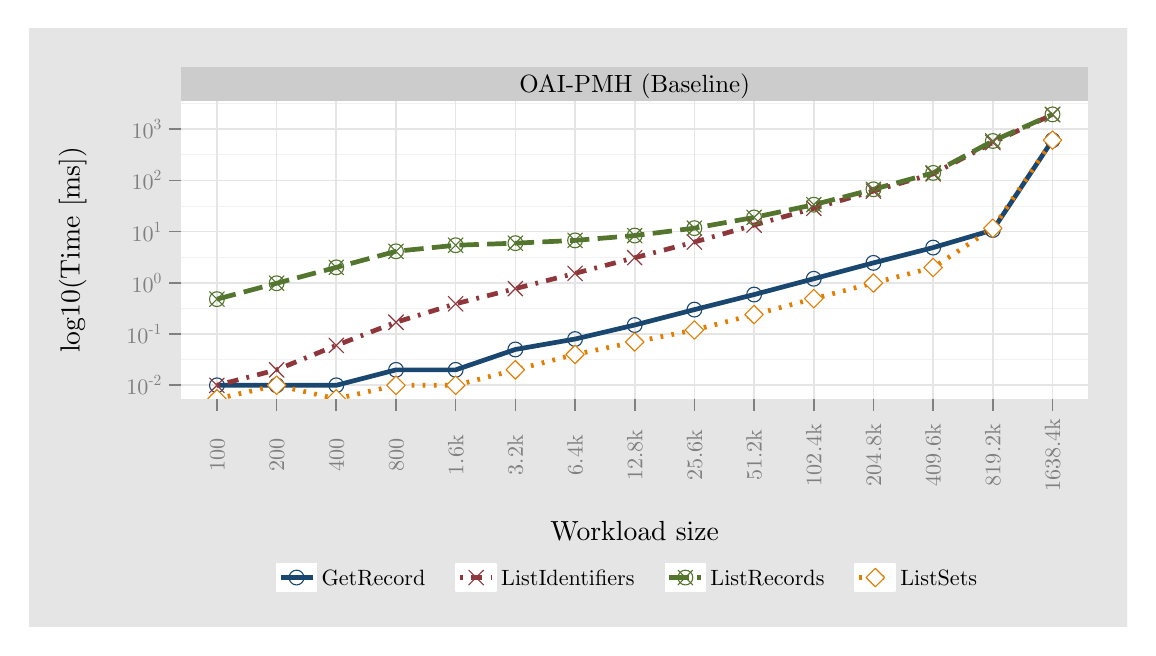
\begin{tikzpicture}[x=1pt,y=1pt]
\definecolor[named]{fillColor}{rgb}{1.00,1.00,1.00}
\path[use as bounding box,fill=fillColor,fill opacity=0.00] (0,0) rectangle (397.48,216.81);
\begin{scope}
\path[clip] (  0.00,  0.00) rectangle (397.48,216.81);
\definecolor[named]{drawColor}{rgb}{1.00,1.00,1.00}
\definecolor[named]{fillColor}{rgb}{0.90,0.90,0.90}

\path[draw=drawColor,line width= 0.6pt,line join=round,line cap=round,fill=fillColor] (  0.00,  0.00) rectangle (397.48,216.81);
\end{scope}
\begin{scope}
\path[clip] ( 55.45, 82.69) rectangle (383.26,190.36);
\definecolor[named]{fillColor}{rgb}{1.00,1.00,1.00}

\path[fill=fillColor] ( 55.45, 82.69) rectangle (383.26,190.36);
\definecolor[named]{drawColor}{rgb}{0.95,0.95,0.95}

\path[draw=drawColor,line width= 0.3pt,line join=round] ( 55.45, 96.84) --
	(383.26, 96.84);

\path[draw=drawColor,line width= 0.3pt,line join=round] ( 55.45,115.36) --
	(383.26,115.36);

\path[draw=drawColor,line width= 0.3pt,line join=round] ( 55.45,133.87) --
	(383.26,133.87);

\path[draw=drawColor,line width= 0.3pt,line join=round] ( 55.45,152.38) --
	(383.26,152.38);

\path[draw=drawColor,line width= 0.3pt,line join=round] ( 55.45,170.90) --
	(383.26,170.90);

\path[draw=drawColor,line width= 0.3pt,line join=round] ( 55.45,189.41) --
	(383.26,189.41);
\definecolor[named]{drawColor}{rgb}{0.90,0.90,0.90}

\path[draw=drawColor,line width= 0.6pt,line join=round] ( 55.45, 87.58) --
	(383.26, 87.58);

\path[draw=drawColor,line width= 0.6pt,line join=round] ( 55.45,106.10) --
	(383.26,106.10);

\path[draw=drawColor,line width= 0.6pt,line join=round] ( 55.45,124.61) --
	(383.26,124.61);

\path[draw=drawColor,line width= 0.6pt,line join=round] ( 55.45,143.13) --
	(383.26,143.13);

\path[draw=drawColor,line width= 0.6pt,line join=round] ( 55.45,161.64) --
	(383.26,161.64);

\path[draw=drawColor,line width= 0.6pt,line join=round] ( 55.45,180.15) --
	(383.26,180.15);

\path[draw=drawColor,line width= 0.6pt,line join=round] ( 68.39, 82.69) --
	( 68.39,190.36);

\path[draw=drawColor,line width= 0.6pt,line join=round] ( 89.95, 82.69) --
	( 89.95,190.36);

\path[draw=drawColor,line width= 0.6pt,line join=round] (111.52, 82.69) --
	(111.52,190.36);

\path[draw=drawColor,line width= 0.6pt,line join=round] (133.09, 82.69) --
	(133.09,190.36);

\path[draw=drawColor,line width= 0.6pt,line join=round] (154.65, 82.69) --
	(154.65,190.36);

\path[draw=drawColor,line width= 0.6pt,line join=round] (176.22, 82.69) --
	(176.22,190.36);

\path[draw=drawColor,line width= 0.6pt,line join=round] (197.79, 82.69) --
	(197.79,190.36);

\path[draw=drawColor,line width= 0.6pt,line join=round] (219.35, 82.69) --
	(219.35,190.36);

\path[draw=drawColor,line width= 0.6pt,line join=round] (240.92, 82.69) --
	(240.92,190.36);

\path[draw=drawColor,line width= 0.6pt,line join=round] (262.49, 82.69) --
	(262.49,190.36);

\path[draw=drawColor,line width= 0.6pt,line join=round] (284.05, 82.69) --
	(284.05,190.36);

\path[draw=drawColor,line width= 0.6pt,line join=round] (305.62, 82.69) --
	(305.62,190.36);

\path[draw=drawColor,line width= 0.6pt,line join=round] (327.19, 82.69) --
	(327.19,190.36);

\path[draw=drawColor,line width= 0.6pt,line join=round] (348.75, 82.69) --
	(348.75,190.36);

\path[draw=drawColor,line width= 0.6pt,line join=round] (370.32, 82.69) --
	(370.32,190.36);
\definecolor[named]{drawColor}{rgb}{0.10,0.28,0.44}

\path[draw=drawColor,line width= 1.7pt,line join=round] ( 68.39, 87.58) --
	( 89.95, 87.58) --
	(111.52, 87.58) --
	(133.09, 93.16) --
	(154.65, 93.16) --
	(176.22,100.53) --
	(197.79,104.30) --
	(219.35,109.36) --
	(240.92,114.93) --
	(262.49,120.37) --
	(284.05,126.08) --
	(305.62,131.82) --
	(327.19,137.34) --
	(348.75,143.68) --
	(370.32,176.15);
\definecolor[named]{drawColor}{rgb}{0.56,0.21,0.23}

\path[draw=drawColor,line width= 1.7pt,dash pattern=on 1pt off 3pt on 4pt off 3pt ,line join=round] ( 68.39, 87.58) --
	( 89.95, 93.16) --
	(111.52,101.99) --
	(133.09,110.36) --
	(154.65,117.04) --
	(176.22,122.51) --
	(197.79,128.03) --
	(219.35,133.68) --
	(240.92,139.35) --
	(262.49,145.47) --
	(284.05,151.53) --
	(305.62,157.78) --
	(327.19,163.99) --
	(348.75,175.32) --
	(370.32,185.41);
\definecolor[named]{drawColor}{rgb}{0.33,0.46,0.18}

\path[draw=drawColor,line width= 1.7pt,dash pattern=on 7pt off 3pt ,line join=round] ( 68.39,118.71) --
	( 89.95,124.45) --
	(111.52,130.19) --
	(133.09,136.00) --
	(154.65,138.19) --
	(176.22,138.94) --
	(197.79,139.94) --
	(219.35,141.69) --
	(240.92,144.37) --
	(262.49,148.24) --
	(284.05,152.84) --
	(305.62,158.41) --
	(327.19,164.33) --
	(348.75,175.86) --
	(370.32,185.47);
\definecolor[named]{drawColor}{rgb}{0.89,0.49,0.00}

\path[draw=drawColor,line width= 1.7pt,dash pattern=on 1pt off 3pt ,line join=round] ( 68.39, 82.69) --
	( 89.95, 87.58) --
	(111.52, 82.69) --
	(133.09, 87.58) --
	(154.65, 87.58) --
	(176.22, 93.16) --
	(197.79, 98.73) --
	(219.35,103.23) --
	(240.92,107.56) --
	(262.49,113.14) --
	(284.05,118.88) --
	(305.62,124.53) --
	(327.19,130.14) --
	(348.75,144.33) --
	(370.32,176.17);
\definecolor[named]{drawColor}{rgb}{0.10,0.28,0.44}

\path[draw=drawColor,line width= 0.4pt,line join=round,line cap=round] ( 68.39, 87.58) circle (  2.67);

\path[draw=drawColor,line width= 0.4pt,line join=round,line cap=round] ( 89.95, 87.58) circle (  2.67);

\path[draw=drawColor,line width= 0.4pt,line join=round,line cap=round] (111.52, 87.58) circle (  2.67);

\path[draw=drawColor,line width= 0.4pt,line join=round,line cap=round] (133.09, 93.16) circle (  2.67);

\path[draw=drawColor,line width= 0.4pt,line join=round,line cap=round] (154.65, 93.16) circle (  2.67);

\path[draw=drawColor,line width= 0.4pt,line join=round,line cap=round] (176.22,100.53) circle (  2.67);

\path[draw=drawColor,line width= 0.4pt,line join=round,line cap=round] (197.79,104.30) circle (  2.67);

\path[draw=drawColor,line width= 0.4pt,line join=round,line cap=round] (219.35,109.36) circle (  2.67);

\path[draw=drawColor,line width= 0.4pt,line join=round,line cap=round] (240.92,114.93) circle (  2.67);

\path[draw=drawColor,line width= 0.4pt,line join=round,line cap=round] (262.49,120.37) circle (  2.67);

\path[draw=drawColor,line width= 0.4pt,line join=round,line cap=round] (284.05,126.08) circle (  2.67);

\path[draw=drawColor,line width= 0.4pt,line join=round,line cap=round] (305.62,131.82) circle (  2.67);

\path[draw=drawColor,line width= 0.4pt,line join=round,line cap=round] (327.19,137.34) circle (  2.67);

\path[draw=drawColor,line width= 0.4pt,line join=round,line cap=round] (348.75,143.68) circle (  2.67);

\path[draw=drawColor,line width= 0.4pt,line join=round,line cap=round] (370.32,176.15) circle (  2.67);
\definecolor[named]{drawColor}{rgb}{0.56,0.21,0.23}

\path[draw=drawColor,line width= 0.4pt,line join=round,line cap=round,fill=fillColor] ( 65.72, 84.92) -- ( 71.06, 90.25);

\path[draw=drawColor,line width= 0.4pt,line join=round,line cap=round,fill=fillColor] ( 65.72, 90.25) -- ( 71.06, 84.92);

\path[draw=drawColor,line width= 0.4pt,line join=round,line cap=round,fill=fillColor] ( 87.29, 90.49) -- ( 92.62, 95.83);

\path[draw=drawColor,line width= 0.4pt,line join=round,line cap=round,fill=fillColor] ( 87.29, 95.83) -- ( 92.62, 90.49);

\path[draw=drawColor,line width= 0.4pt,line join=round,line cap=round,fill=fillColor] (108.85, 99.32) -- (114.19,104.66);

\path[draw=drawColor,line width= 0.4pt,line join=round,line cap=round,fill=fillColor] (108.85,104.66) -- (114.19, 99.32);

\path[draw=drawColor,line width= 0.4pt,line join=round,line cap=round,fill=fillColor] (130.42,107.70) -- (135.76,113.03);

\path[draw=drawColor,line width= 0.4pt,line join=round,line cap=round,fill=fillColor] (130.42,113.03) -- (135.76,107.70);

\path[draw=drawColor,line width= 0.4pt,line join=round,line cap=round,fill=fillColor] (151.99,114.37) -- (157.32,119.71);

\path[draw=drawColor,line width= 0.4pt,line join=round,line cap=round,fill=fillColor] (151.99,119.71) -- (157.32,114.37);

\path[draw=drawColor,line width= 0.4pt,line join=round,line cap=round,fill=fillColor] (173.55,119.84) -- (178.89,125.18);

\path[draw=drawColor,line width= 0.4pt,line join=round,line cap=round,fill=fillColor] (173.55,125.18) -- (178.89,119.84);

\path[draw=drawColor,line width= 0.4pt,line join=round,line cap=round,fill=fillColor] (195.12,125.36) -- (200.45,130.70);

\path[draw=drawColor,line width= 0.4pt,line join=round,line cap=round,fill=fillColor] (195.12,130.70) -- (200.45,125.36);

\path[draw=drawColor,line width= 0.4pt,line join=round,line cap=round,fill=fillColor] (216.69,131.02) -- (222.02,136.35);

\path[draw=drawColor,line width= 0.4pt,line join=round,line cap=round,fill=fillColor] (216.69,136.35) -- (222.02,131.02);

\path[draw=drawColor,line width= 0.4pt,line join=round,line cap=round,fill=fillColor] (238.25,136.68) -- (243.59,142.01);

\path[draw=drawColor,line width= 0.4pt,line join=round,line cap=round,fill=fillColor] (238.25,142.01) -- (243.59,136.68);

\path[draw=drawColor,line width= 0.4pt,line join=round,line cap=round,fill=fillColor] (259.82,142.80) -- (265.15,148.13);

\path[draw=drawColor,line width= 0.4pt,line join=round,line cap=round,fill=fillColor] (259.82,148.13) -- (265.15,142.80);

\path[draw=drawColor,line width= 0.4pt,line join=round,line cap=round,fill=fillColor] (281.39,148.87) -- (286.72,154.20);

\path[draw=drawColor,line width= 0.4pt,line join=round,line cap=round,fill=fillColor] (281.39,154.20) -- (286.72,148.87);

\path[draw=drawColor,line width= 0.4pt,line join=round,line cap=round,fill=fillColor] (302.95,155.11) -- (308.29,160.44);

\path[draw=drawColor,line width= 0.4pt,line join=round,line cap=round,fill=fillColor] (302.95,160.44) -- (308.29,155.11);

\path[draw=drawColor,line width= 0.4pt,line join=round,line cap=round,fill=fillColor] (324.52,161.32) -- (329.85,166.66);

\path[draw=drawColor,line width= 0.4pt,line join=round,line cap=round,fill=fillColor] (324.52,166.66) -- (329.85,161.32);

\path[draw=drawColor,line width= 0.4pt,line join=round,line cap=round,fill=fillColor] (346.08,172.65) -- (351.42,177.98);

\path[draw=drawColor,line width= 0.4pt,line join=round,line cap=round,fill=fillColor] (346.08,177.98) -- (351.42,172.65);

\path[draw=drawColor,line width= 0.4pt,line join=round,line cap=round,fill=fillColor] (367.65,182.74) -- (372.99,188.08);

\path[draw=drawColor,line width= 0.4pt,line join=round,line cap=round,fill=fillColor] (367.65,188.08) -- (372.99,182.74);
\definecolor[named]{drawColor}{rgb}{0.33,0.46,0.18}

\path[draw=drawColor,line width= 0.4pt,line join=round,line cap=round] ( 68.39,118.71) circle (  2.67);

\path[draw=drawColor,line width= 0.4pt,line join=round,line cap=round] ( 65.72,116.04) -- ( 71.06,121.38);

\path[draw=drawColor,line width= 0.4pt,line join=round,line cap=round] ( 65.72,121.38) -- ( 71.06,116.04);

\path[draw=drawColor,line width= 0.4pt,line join=round,line cap=round] ( 89.95,124.45) circle (  2.67);

\path[draw=drawColor,line width= 0.4pt,line join=round,line cap=round] ( 87.29,121.78) -- ( 92.62,127.12);

\path[draw=drawColor,line width= 0.4pt,line join=round,line cap=round] ( 87.29,127.12) -- ( 92.62,121.78);

\path[draw=drawColor,line width= 0.4pt,line join=round,line cap=round] (111.52,130.19) circle (  2.67);

\path[draw=drawColor,line width= 0.4pt,line join=round,line cap=round] (108.85,127.52) -- (114.19,132.85);

\path[draw=drawColor,line width= 0.4pt,line join=round,line cap=round] (108.85,132.85) -- (114.19,127.52);

\path[draw=drawColor,line width= 0.4pt,line join=round,line cap=round] (133.09,136.00) circle (  2.67);

\path[draw=drawColor,line width= 0.4pt,line join=round,line cap=round] (130.42,133.33) -- (135.76,138.66);

\path[draw=drawColor,line width= 0.4pt,line join=round,line cap=round] (130.42,138.66) -- (135.76,133.33);

\path[draw=drawColor,line width= 0.4pt,line join=round,line cap=round] (154.65,138.19) circle (  2.67);

\path[draw=drawColor,line width= 0.4pt,line join=round,line cap=round] (151.99,135.52) -- (157.32,140.85);

\path[draw=drawColor,line width= 0.4pt,line join=round,line cap=round] (151.99,140.85) -- (157.32,135.52);

\path[draw=drawColor,line width= 0.4pt,line join=round,line cap=round] (176.22,138.94) circle (  2.67);

\path[draw=drawColor,line width= 0.4pt,line join=round,line cap=round] (173.55,136.27) -- (178.89,141.60);

\path[draw=drawColor,line width= 0.4pt,line join=round,line cap=round] (173.55,141.60) -- (178.89,136.27);

\path[draw=drawColor,line width= 0.4pt,line join=round,line cap=round] (197.79,139.94) circle (  2.67);

\path[draw=drawColor,line width= 0.4pt,line join=round,line cap=round] (195.12,137.27) -- (200.45,142.61);

\path[draw=drawColor,line width= 0.4pt,line join=round,line cap=round] (195.12,142.61) -- (200.45,137.27);

\path[draw=drawColor,line width= 0.4pt,line join=round,line cap=round] (219.35,141.69) circle (  2.67);

\path[draw=drawColor,line width= 0.4pt,line join=round,line cap=round] (216.69,139.03) -- (222.02,144.36);

\path[draw=drawColor,line width= 0.4pt,line join=round,line cap=round] (216.69,144.36) -- (222.02,139.03);

\path[draw=drawColor,line width= 0.4pt,line join=round,line cap=round] (240.92,144.37) circle (  2.67);

\path[draw=drawColor,line width= 0.4pt,line join=round,line cap=round] (238.25,141.71) -- (243.59,147.04);

\path[draw=drawColor,line width= 0.4pt,line join=round,line cap=round] (238.25,147.04) -- (243.59,141.71);

\path[draw=drawColor,line width= 0.4pt,line join=round,line cap=round] (262.49,148.24) circle (  2.67);

\path[draw=drawColor,line width= 0.4pt,line join=round,line cap=round] (259.82,145.58) -- (265.15,150.91);

\path[draw=drawColor,line width= 0.4pt,line join=round,line cap=round] (259.82,150.91) -- (265.15,145.58);

\path[draw=drawColor,line width= 0.4pt,line join=round,line cap=round] (284.05,152.84) circle (  2.67);

\path[draw=drawColor,line width= 0.4pt,line join=round,line cap=round] (281.39,150.17) -- (286.72,155.50);

\path[draw=drawColor,line width= 0.4pt,line join=round,line cap=round] (281.39,155.50) -- (286.72,150.17);

\path[draw=drawColor,line width= 0.4pt,line join=round,line cap=round] (305.62,158.41) circle (  2.67);

\path[draw=drawColor,line width= 0.4pt,line join=round,line cap=round] (302.95,155.75) -- (308.29,161.08);

\path[draw=drawColor,line width= 0.4pt,line join=round,line cap=round] (302.95,161.08) -- (308.29,155.75);

\path[draw=drawColor,line width= 0.4pt,line join=round,line cap=round] (327.19,164.33) circle (  2.67);

\path[draw=drawColor,line width= 0.4pt,line join=round,line cap=round] (324.52,161.66) -- (329.85,167.00);

\path[draw=drawColor,line width= 0.4pt,line join=round,line cap=round] (324.52,167.00) -- (329.85,161.66);

\path[draw=drawColor,line width= 0.4pt,line join=round,line cap=round] (348.75,175.86) circle (  2.67);

\path[draw=drawColor,line width= 0.4pt,line join=round,line cap=round] (346.08,173.19) -- (351.42,178.53);

\path[draw=drawColor,line width= 0.4pt,line join=round,line cap=round] (346.08,178.53) -- (351.42,173.19);

\path[draw=drawColor,line width= 0.4pt,line join=round,line cap=round] (370.32,185.47) circle (  2.67);

\path[draw=drawColor,line width= 0.4pt,line join=round,line cap=round] (367.65,182.80) -- (372.99,188.14);

\path[draw=drawColor,line width= 0.4pt,line join=round,line cap=round] (367.65,188.14) -- (372.99,182.80);
\definecolor[named]{drawColor}{rgb}{0.89,0.49,0.00}

\path[draw=drawColor,line width= 0.4pt,line join=round,line cap=round,fill=fillColor] ( 68.39, 79.35) --
	( 71.73, 82.69) --
	( 68.39, 86.03) --
	( 65.05, 82.69) --
	cycle;

\path[draw=drawColor,line width= 0.4pt,line join=round,line cap=round,fill=fillColor] ( 89.95, 84.24) --
	( 93.30, 87.58) --
	( 89.95, 90.93) --
	( 86.61, 87.58) --
	cycle;

\path[draw=drawColor,line width= 0.4pt,line join=round,line cap=round,fill=fillColor] (111.52, 79.35) --
	(114.86, 82.69) --
	(111.52, 86.03) --
	(108.18, 82.69) --
	cycle;

\path[draw=drawColor,line width= 0.4pt,line join=round,line cap=round,fill=fillColor] (133.09, 84.24) --
	(136.43, 87.58) --
	(133.09, 90.93) --
	(129.74, 87.58) --
	cycle;

\path[draw=drawColor,line width= 0.4pt,line join=round,line cap=round,fill=fillColor] (154.65, 84.24) --
	(158.00, 87.58) --
	(154.65, 90.93) --
	(151.31, 87.58) --
	cycle;

\path[draw=drawColor,line width= 0.4pt,line join=round,line cap=round,fill=fillColor] (176.22, 89.81) --
	(179.56, 93.16) --
	(176.22, 96.50) --
	(172.88, 93.16) --
	cycle;

\path[draw=drawColor,line width= 0.4pt,line join=round,line cap=round,fill=fillColor] (197.79, 95.39) --
	(201.13, 98.73) --
	(197.79,102.07) --
	(194.44, 98.73) --
	cycle;

\path[draw=drawColor,line width= 0.4pt,line join=round,line cap=round,fill=fillColor] (219.35, 99.89) --
	(222.70,103.23) --
	(219.35,106.57) --
	(216.01,103.23) --
	cycle;

\path[draw=drawColor,line width= 0.4pt,line join=round,line cap=round,fill=fillColor] (240.92,104.22) --
	(244.26,107.56) --
	(240.92,110.91) --
	(237.58,107.56) --
	cycle;

\path[draw=drawColor,line width= 0.4pt,line join=round,line cap=round,fill=fillColor] (262.49,109.79) --
	(265.83,113.14) --
	(262.49,116.48) --
	(259.14,113.14) --
	cycle;

\path[draw=drawColor,line width= 0.4pt,line join=round,line cap=round,fill=fillColor] (284.05,115.53) --
	(287.40,118.88) --
	(284.05,122.22) --
	(280.71,118.88) --
	cycle;

\path[draw=drawColor,line width= 0.4pt,line join=round,line cap=round,fill=fillColor] (305.62,121.19) --
	(308.96,124.53) --
	(305.62,127.87) --
	(302.28,124.53) --
	cycle;

\path[draw=drawColor,line width= 0.4pt,line join=round,line cap=round,fill=fillColor] (327.19,126.80) --
	(330.53,130.14) --
	(327.19,133.49) --
	(323.84,130.14) --
	cycle;

\path[draw=drawColor,line width= 0.4pt,line join=round,line cap=round,fill=fillColor] (348.75,140.98) --
	(352.10,144.33) --
	(348.75,147.67) --
	(345.41,144.33) --
	cycle;

\path[draw=drawColor,line width= 0.4pt,line join=round,line cap=round,fill=fillColor] (370.32,172.82) --
	(373.66,176.17) --
	(370.32,179.51) --
	(366.98,176.17) --
	cycle;
\end{scope}
\begin{scope}
\path[clip] (  0.00,  0.00) rectangle (397.48,216.81);
\definecolor[named]{fillColor}{rgb}{0.80,0.80,0.80}

\path[fill=fillColor] ( 55.45,190.36) rectangle (383.26,202.58);
\definecolor[named]{drawColor}{rgb}{0.00,0.00,0.00}

\node[text=drawColor,anchor=base,inner sep=0pt, outer sep=0pt, scale=  0.90] at (219.35,193.37) {OAI-PMH (Baseline)};
\end{scope}
\begin{scope}
\path[clip] (  0.00,  0.00) rectangle (397.48,216.81);
\definecolor[named]{drawColor}{rgb}{0.50,0.50,0.50}

\node[text=drawColor,anchor=base west,inner sep=0pt, outer sep=0pt, scale=  0.80] at ( 35.67, 84.15) {10};

\node[text=drawColor,anchor=base west,inner sep=0pt, outer sep=0pt, scale=  0.56] at ( 43.67, 87.42) {-};

\node[text=drawColor,anchor=base west,inner sep=0pt, outer sep=0pt, scale=  0.56] at ( 45.54, 87.42) {2};

\node[text=drawColor,anchor=base west,inner sep=0pt, outer sep=0pt, scale=  0.80] at ( 35.67,102.67) {10};

\node[text=drawColor,anchor=base west,inner sep=0pt, outer sep=0pt, scale=  0.56] at ( 43.67,105.94) {-};

\node[text=drawColor,anchor=base west,inner sep=0pt, outer sep=0pt, scale=  0.56] at ( 45.54,105.94) {1};

\node[text=drawColor,anchor=base west,inner sep=0pt, outer sep=0pt, scale=  0.80] at ( 37.54,121.18) {10};

\node[text=drawColor,anchor=base west,inner sep=0pt, outer sep=0pt, scale=  0.56] at ( 45.54,124.45) {0};

\node[text=drawColor,anchor=base west,inner sep=0pt, outer sep=0pt, scale=  0.80] at ( 37.54,139.69) {10};

\node[text=drawColor,anchor=base west,inner sep=0pt, outer sep=0pt, scale=  0.56] at ( 45.54,142.96) {1};

\node[text=drawColor,anchor=base west,inner sep=0pt, outer sep=0pt, scale=  0.80] at ( 37.54,158.21) {10};

\node[text=drawColor,anchor=base west,inner sep=0pt, outer sep=0pt, scale=  0.56] at ( 45.54,161.48) {2};

\node[text=drawColor,anchor=base west,inner sep=0pt, outer sep=0pt, scale=  0.80] at ( 37.54,176.72) {10};

\node[text=drawColor,anchor=base west,inner sep=0pt, outer sep=0pt, scale=  0.56] at ( 45.54,179.99) {3};
\end{scope}
\begin{scope}
\path[clip] (  0.00,  0.00) rectangle (397.48,216.81);
\definecolor[named]{drawColor}{rgb}{0.50,0.50,0.50}

\path[draw=drawColor,line width= 0.6pt,line join=round] ( 51.18, 87.58) --
	( 55.45, 87.58);

\path[draw=drawColor,line width= 0.6pt,line join=round] ( 51.18,106.10) --
	( 55.45,106.10);

\path[draw=drawColor,line width= 0.6pt,line join=round] ( 51.18,124.61) --
	( 55.45,124.61);

\path[draw=drawColor,line width= 0.6pt,line join=round] ( 51.18,143.13) --
	( 55.45,143.13);

\path[draw=drawColor,line width= 0.6pt,line join=round] ( 51.18,161.64) --
	( 55.45,161.64);

\path[draw=drawColor,line width= 0.6pt,line join=round] ( 51.18,180.15) --
	( 55.45,180.15);
\end{scope}
\begin{scope}
\path[clip] (  0.00,  0.00) rectangle (397.48,216.81);
\definecolor[named]{drawColor}{rgb}{0.50,0.50,0.50}

\path[draw=drawColor,line width= 0.6pt,line join=round] ( 68.39, 78.42) --
	( 68.39, 82.69);

\path[draw=drawColor,line width= 0.6pt,line join=round] ( 89.95, 78.42) --
	( 89.95, 82.69);

\path[draw=drawColor,line width= 0.6pt,line join=round] (111.52, 78.42) --
	(111.52, 82.69);

\path[draw=drawColor,line width= 0.6pt,line join=round] (133.09, 78.42) --
	(133.09, 82.69);

\path[draw=drawColor,line width= 0.6pt,line join=round] (154.65, 78.42) --
	(154.65, 82.69);

\path[draw=drawColor,line width= 0.6pt,line join=round] (176.22, 78.42) --
	(176.22, 82.69);

\path[draw=drawColor,line width= 0.6pt,line join=round] (197.79, 78.42) --
	(197.79, 82.69);

\path[draw=drawColor,line width= 0.6pt,line join=round] (219.35, 78.42) --
	(219.35, 82.69);

\path[draw=drawColor,line width= 0.6pt,line join=round] (240.92, 78.42) --
	(240.92, 82.69);

\path[draw=drawColor,line width= 0.6pt,line join=round] (262.49, 78.42) --
	(262.49, 82.69);

\path[draw=drawColor,line width= 0.6pt,line join=round] (284.05, 78.42) --
	(284.05, 82.69);

\path[draw=drawColor,line width= 0.6pt,line join=round] (305.62, 78.42) --
	(305.62, 82.69);

\path[draw=drawColor,line width= 0.6pt,line join=round] (327.19, 78.42) --
	(327.19, 82.69);

\path[draw=drawColor,line width= 0.6pt,line join=round] (348.75, 78.42) --
	(348.75, 82.69);

\path[draw=drawColor,line width= 0.6pt,line join=round] (370.32, 78.42) --
	(370.32, 82.69);
\end{scope}
\begin{scope}
\path[clip] (  0.00,  0.00) rectangle (397.48,216.81);
\definecolor[named]{drawColor}{rgb}{0.50,0.50,0.50}

\node[text=drawColor,rotate= 90.00,anchor=base,inner sep=0pt, outer sep=0pt, scale=  0.80] at ( 71.14, 62.36) {100};

\node[text=drawColor,rotate= 90.00,anchor=base,inner sep=0pt, outer sep=0pt, scale=  0.80] at ( 92.71, 62.36) {200};

\node[text=drawColor,rotate= 90.00,anchor=base,inner sep=0pt, outer sep=0pt, scale=  0.80] at (114.28, 62.36) {400};

\node[text=drawColor,rotate= 90.00,anchor=base,inner sep=0pt, outer sep=0pt, scale=  0.80] at (135.84, 62.36) {800};

\node[text=drawColor,rotate= 90.00,anchor=base,inner sep=0pt, outer sep=0pt, scale=  0.80] at (157.41, 62.36) {1.6k};

\node[text=drawColor,rotate= 90.00,anchor=base,inner sep=0pt, outer sep=0pt, scale=  0.80] at (178.98, 62.36) {3.2k};

\node[text=drawColor,rotate= 90.00,anchor=base,inner sep=0pt, outer sep=0pt, scale=  0.80] at (200.54, 62.36) {6.4k};

\node[text=drawColor,rotate= 90.00,anchor=base,inner sep=0pt, outer sep=0pt, scale=  0.80] at (222.11, 62.36) {12.8k};

\node[text=drawColor,rotate= 90.00,anchor=base,inner sep=0pt, outer sep=0pt, scale=  0.80] at (243.67, 62.36) {25.6k};

\node[text=drawColor,rotate= 90.00,anchor=base,inner sep=0pt, outer sep=0pt, scale=  0.80] at (265.24, 62.36) {51.2k};

\node[text=drawColor,rotate= 90.00,anchor=base,inner sep=0pt, outer sep=0pt, scale=  0.80] at (286.81, 62.36) {102.4k};

\node[text=drawColor,rotate= 90.00,anchor=base,inner sep=0pt, outer sep=0pt, scale=  0.80] at (308.37, 62.36) {204.8k};

\node[text=drawColor,rotate= 90.00,anchor=base,inner sep=0pt, outer sep=0pt, scale=  0.80] at (329.94, 62.36) {409.6k};

\node[text=drawColor,rotate= 90.00,anchor=base,inner sep=0pt, outer sep=0pt, scale=  0.80] at (351.51, 62.36) {819.2k};

\node[text=drawColor,rotate= 90.00,anchor=base,inner sep=0pt, outer sep=0pt, scale=  0.80] at (373.07, 62.36) {1638.4k};
\end{scope}
\begin{scope}
\path[clip] (  0.00,  0.00) rectangle (397.48,216.81);
\definecolor[named]{drawColor}{rgb}{0.00,0.00,0.00}

\node[text=drawColor,anchor=base,inner sep=0pt, outer sep=0pt, scale=  1.00] at (219.35, 31.41) {Workload size};
\end{scope}
\begin{scope}
\path[clip] (  0.00,  0.00) rectangle (397.48,216.81);
\definecolor[named]{drawColor}{rgb}{0.00,0.00,0.00}

\node[text=drawColor,rotate= 90.00,anchor=base,inner sep=0pt, outer sep=0pt, scale=  1.00] at ( 18.80,136.53) {log10(Time [ms])};
\end{scope}
\begin{scope}
\path[clip] (  0.00,  0.00) rectangle (397.48,216.81);
\definecolor[named]{fillColor}{rgb}{0.90,0.90,0.90}

\path[fill=fillColor] ( 82.04,  8.87) rectangle (356.67, 27.36);
\end{scope}
\begin{scope}
\path[clip] (  0.00,  0.00) rectangle (397.48,216.81);
\definecolor[named]{drawColor}{rgb}{1.00,1.00,1.00}
\definecolor[named]{fillColor}{rgb}{1.00,1.00,1.00}

\path[draw=drawColor,line width= 0.6pt,line join=round,line cap=round,fill=fillColor] ( 89.92, 13.14) rectangle (104.38, 23.09);
\end{scope}
\begin{scope}
\path[clip] (  0.00,  0.00) rectangle (397.48,216.81);
\definecolor[named]{drawColor}{rgb}{0.10,0.28,0.44}

\path[draw=drawColor,line width= 1.7pt,line join=round] ( 91.37, 18.11) -- (102.93, 18.11);
\end{scope}
\begin{scope}
\path[clip] (  0.00,  0.00) rectangle (397.48,216.81);
\definecolor[named]{drawColor}{rgb}{0.10,0.28,0.44}

\path[draw=drawColor,line width= 0.4pt,line join=round,line cap=round] ( 97.15, 18.11) circle (  2.67);
\end{scope}
\begin{scope}
\path[clip] (  0.00,  0.00) rectangle (397.48,216.81);
\definecolor[named]{drawColor}{rgb}{1.00,1.00,1.00}
\definecolor[named]{fillColor}{rgb}{1.00,1.00,1.00}

\path[draw=drawColor,line width= 0.6pt,line join=round,line cap=round,fill=fillColor] (154.83, 13.14) rectangle (169.29, 23.09);
\end{scope}
\begin{scope}
\path[clip] (  0.00,  0.00) rectangle (397.48,216.81);
\definecolor[named]{drawColor}{rgb}{0.56,0.21,0.23}

\path[draw=drawColor,line width= 1.7pt,dash pattern=on 1pt off 3pt on 4pt off 3pt ,line join=round] (156.28, 18.11) -- (167.84, 18.11);
\end{scope}
\begin{scope}
\path[clip] (  0.00,  0.00) rectangle (397.48,216.81);
\definecolor[named]{drawColor}{rgb}{0.56,0.21,0.23}
\definecolor[named]{fillColor}{rgb}{1.00,1.00,1.00}

\path[draw=drawColor,line width= 0.4pt,line join=round,line cap=round,fill=fillColor] (159.39, 15.45) -- (164.73, 20.78);

\path[draw=drawColor,line width= 0.4pt,line join=round,line cap=round,fill=fillColor] (159.39, 20.78) -- (164.73, 15.45);
\end{scope}
\begin{scope}
\path[clip] (  0.00,  0.00) rectangle (397.48,216.81);
\definecolor[named]{drawColor}{rgb}{1.00,1.00,1.00}
\definecolor[named]{fillColor}{rgb}{1.00,1.00,1.00}

\path[draw=drawColor,line width= 0.6pt,line join=round,line cap=round,fill=fillColor] (230.45, 13.14) rectangle (244.90, 23.09);
\end{scope}
\begin{scope}
\path[clip] (  0.00,  0.00) rectangle (397.48,216.81);
\definecolor[named]{drawColor}{rgb}{0.33,0.46,0.18}

\path[draw=drawColor,line width= 1.7pt,dash pattern=on 7pt off 3pt ,line join=round] (231.89, 18.11) -- (243.45, 18.11);
\end{scope}
\begin{scope}
\path[clip] (  0.00,  0.00) rectangle (397.48,216.81);
\definecolor[named]{drawColor}{rgb}{0.33,0.46,0.18}

\path[draw=drawColor,line width= 0.4pt,line join=round,line cap=round] (237.67, 18.11) circle (  2.67);

\path[draw=drawColor,line width= 0.4pt,line join=round,line cap=round] (235.00, 15.45) -- (240.34, 20.78);

\path[draw=drawColor,line width= 0.4pt,line join=round,line cap=round] (235.00, 20.78) -- (240.34, 15.45);
\end{scope}
\begin{scope}
\path[clip] (  0.00,  0.00) rectangle (397.48,216.81);
\definecolor[named]{drawColor}{rgb}{1.00,1.00,1.00}
\definecolor[named]{fillColor}{rgb}{1.00,1.00,1.00}

\path[draw=drawColor,line width= 0.6pt,line join=round,line cap=round,fill=fillColor] (299.06, 13.14) rectangle (313.51, 23.09);
\end{scope}
\begin{scope}
\path[clip] (  0.00,  0.00) rectangle (397.48,216.81);
\definecolor[named]{drawColor}{rgb}{0.89,0.49,0.00}

\path[draw=drawColor,line width= 1.7pt,dash pattern=on 1pt off 3pt ,line join=round] (300.50, 18.11) -- (312.07, 18.11);
\end{scope}
\begin{scope}
\path[clip] (  0.00,  0.00) rectangle (397.48,216.81);
\definecolor[named]{drawColor}{rgb}{0.89,0.49,0.00}
\definecolor[named]{fillColor}{rgb}{1.00,1.00,1.00}

\path[draw=drawColor,line width= 0.4pt,line join=round,line cap=round,fill=fillColor] (306.28, 14.77) --
	(309.63, 18.11) --
	(306.28, 21.46) --
	(302.94, 18.11) --
	cycle;
\end{scope}
\begin{scope}
\path[clip] (  0.00,  0.00) rectangle (397.48,216.81);
\definecolor[named]{drawColor}{rgb}{0.00,0.00,0.00}

\node[text=drawColor,anchor=base west,inner sep=0pt, outer sep=0pt, scale=  0.80] at (106.18, 15.36) {GetRecord $\;\;\;$};
\end{scope}
\begin{scope}
\path[clip] (  0.00,  0.00) rectangle (397.48,216.81);
\definecolor[named]{drawColor}{rgb}{0.00,0.00,0.00}

\node[text=drawColor,anchor=base west,inner sep=0pt, outer sep=0pt, scale=  0.80] at (171.10, 15.36) {ListIdentifiers $\;\;\;$};
\end{scope}
\begin{scope}
\path[clip] (  0.00,  0.00) rectangle (397.48,216.81);
\definecolor[named]{drawColor}{rgb}{0.00,0.00,0.00}

\node[text=drawColor,anchor=base west,inner sep=0pt, outer sep=0pt, scale=  0.80] at (246.71, 15.36) {ListRecords $\;\;\;$};
\end{scope}
\begin{scope}
\path[clip] (  0.00,  0.00) rectangle (397.48,216.81);
\definecolor[named]{drawColor}{rgb}{0.00,0.00,0.00}

\node[text=drawColor,anchor=base west,inner sep=0pt, outer sep=0pt, scale=  0.80] at (315.32, 15.36) {ListSets $\;\;\;$};
\end{scope}
\end{tikzpicture}
